% 19 日の Oliver（と Meisam）との会議用まとめの日本語版（自分の理解用）と、話す順番。
% 英語版 meeting_1019_summary.tex と同じ内容・同じ図。
% ビルド: lualatex meeting_1019_summary_ja.tex （2回）
\documentclass[11pt,a4paper]{article}
\usepackage{luatexja}
\usepackage[margin=2cm]{geometry}
\usepackage{amsmath,amssymb}
\usepackage{enumitem}
\usepackage{graphicx}
\usepackage{tabularx,booktabs}
\graphicspath{{assets/}}
\setlist{nosep,leftmargin=*}
\pagestyle{empty}
\begin{document}
\begin{center}
{\large\bfseries Gauss 点での場と点モデルのつなぎ方（日本語版）}\\[2pt]
西岡佳祐、2026 年 10 月 19 日の会議用（自分の理解用。英語版と同じ内容）
\end{center}

\paragraph{今の状況。} 修論は書き終わっていて、11 月中旬に提出する予定（コロキウムは 12 月 16 日）。
点モデルは Klempt et al. のハミルトン原理の点モデルで、種間作用のパラメータは Heine et al. の
in vitro のデータからベイズ推定（TMCMC）で決めた。機械学習ではない。

\paragraph{1. Gauss 点での $\phi_{3D}$。} 要素は場を NEM で Gauss 点と表面の点で直接解くので、
各 Gauss 点で $\phi_{3D}$ が補間なしに分かる。点モデルは各 Gauss 点で、場の横で解いている。

\paragraph{2. 二つの空隙：二つの方式を実装した。}（修論では (a) を scaled、(b) を unscaled と呼んでいる。）
場の空隙（$1-\phi_{3D}$）と点モデルの空隙（$\phi_0$）は別のもの。これをどうそろえるかで方式が分かれる。
\begin{itemize}
\item \emph{(a) 量で成長（growth from the amount）。} 量は場、点モデルは組成 $\phi_i/\sum_j\phi_j$ と生きた割合 $\psi_i$ だけを決める。
  各 Gauss 点・各刻みで、点モデルの状態を $\sum_i\phi_i=\phi_{3D}$ に縮めてから進め、また戻す。
  すると $\phi_0=1-\phi_{3D}$ となり、$\phi_0$ に「場の空隙」という物理的な意味を持たせることになる。
  場の量が点モデル自身の量と同じときは、点モデル単独の組成を $10^{-5}$ 以内で再現する。
\item \emph{(b) 独立した点モデル（free point model）。} $\phi_0$ は論文どおり補助の変数のまま。場がしきい値に届いた時点から
  点モデルが自分だけで進み、組成だけを渡す。
\end{itemize}
組成は、(a) では「その場所の量」で、(b) では「その場所のバイオフィルムの年齢（できてからの時間）」で決まる。

\noindent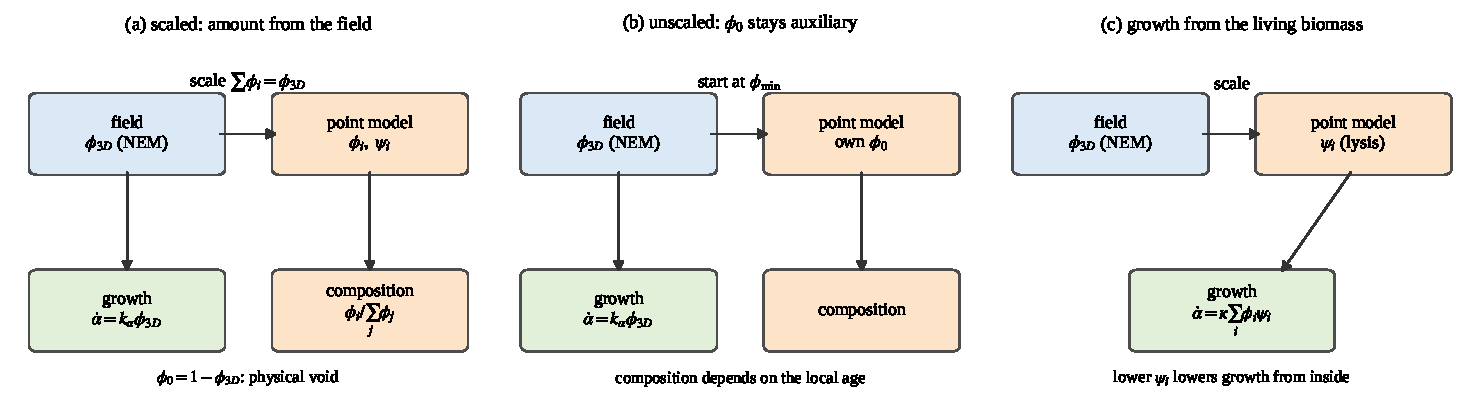
\includegraphics[width=\linewidth]{fig_meeting1019_schemes.pdf}\\
{\small Gauss 点でのつなぎ方：(a) 量で成長、(b) 独立した点モデル、(c) 点モデルの生きている量で成長。}

\noindent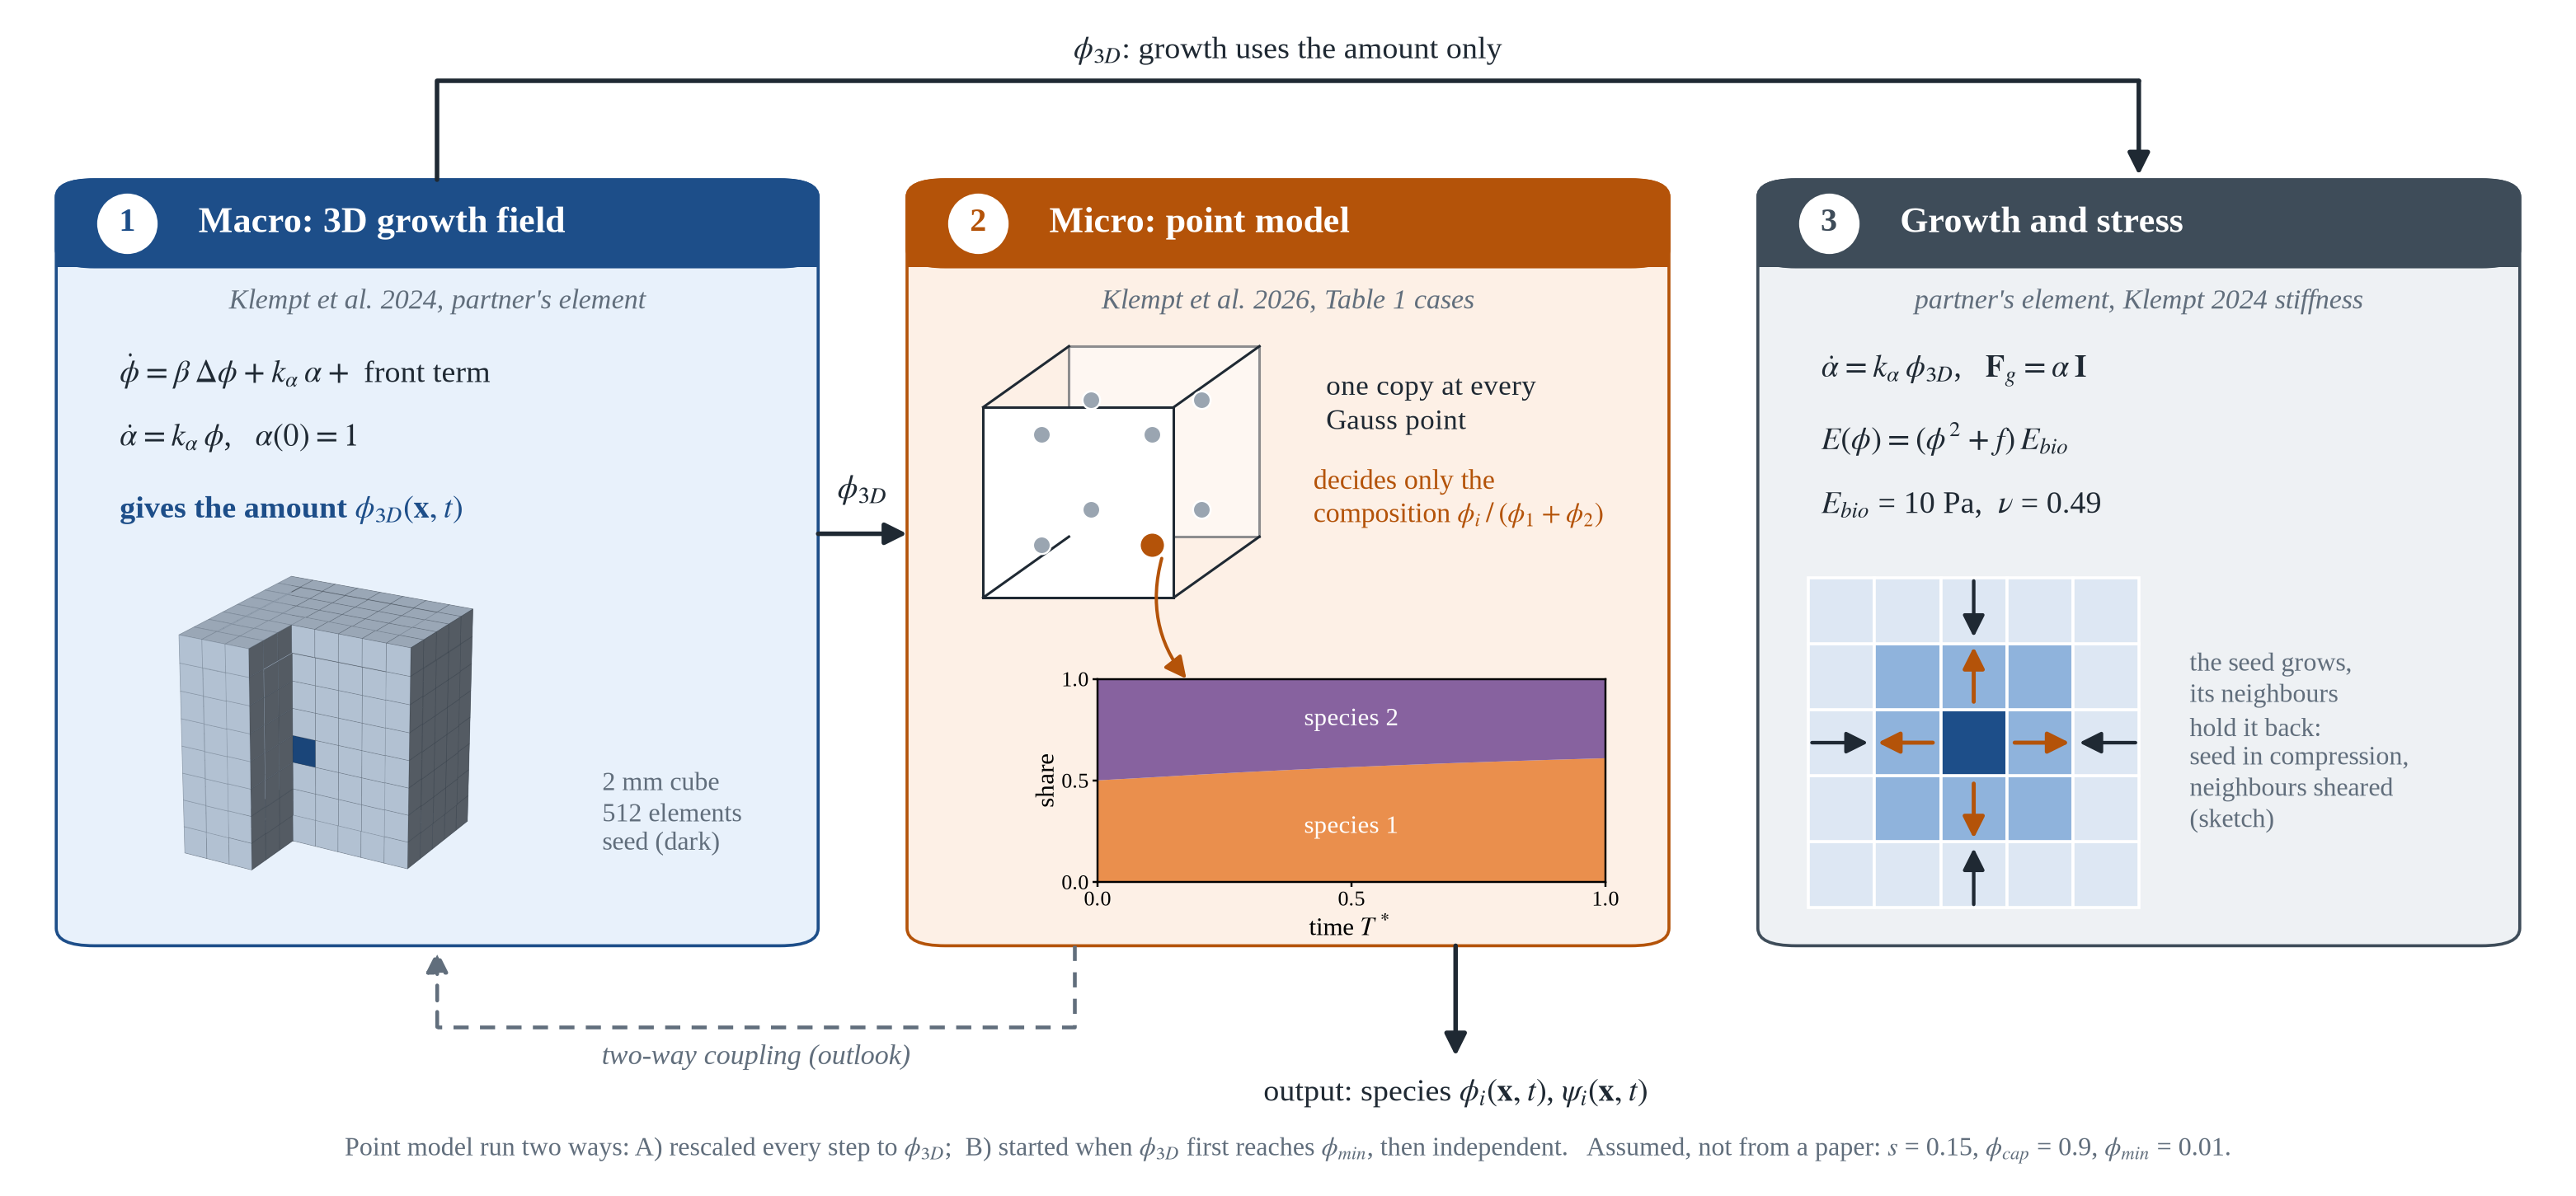
\includegraphics[width=\linewidth]{fig_coupling_schematic.png}\\
{\small 方式 (a)（修論と同じ。図は 2 菌種）：場が量 $\phi_{3D}$ を、各 Gauss 点の点モデルが組成だけを決め、成長と応力は $\phi_{3D}$ を使う。}

\noindent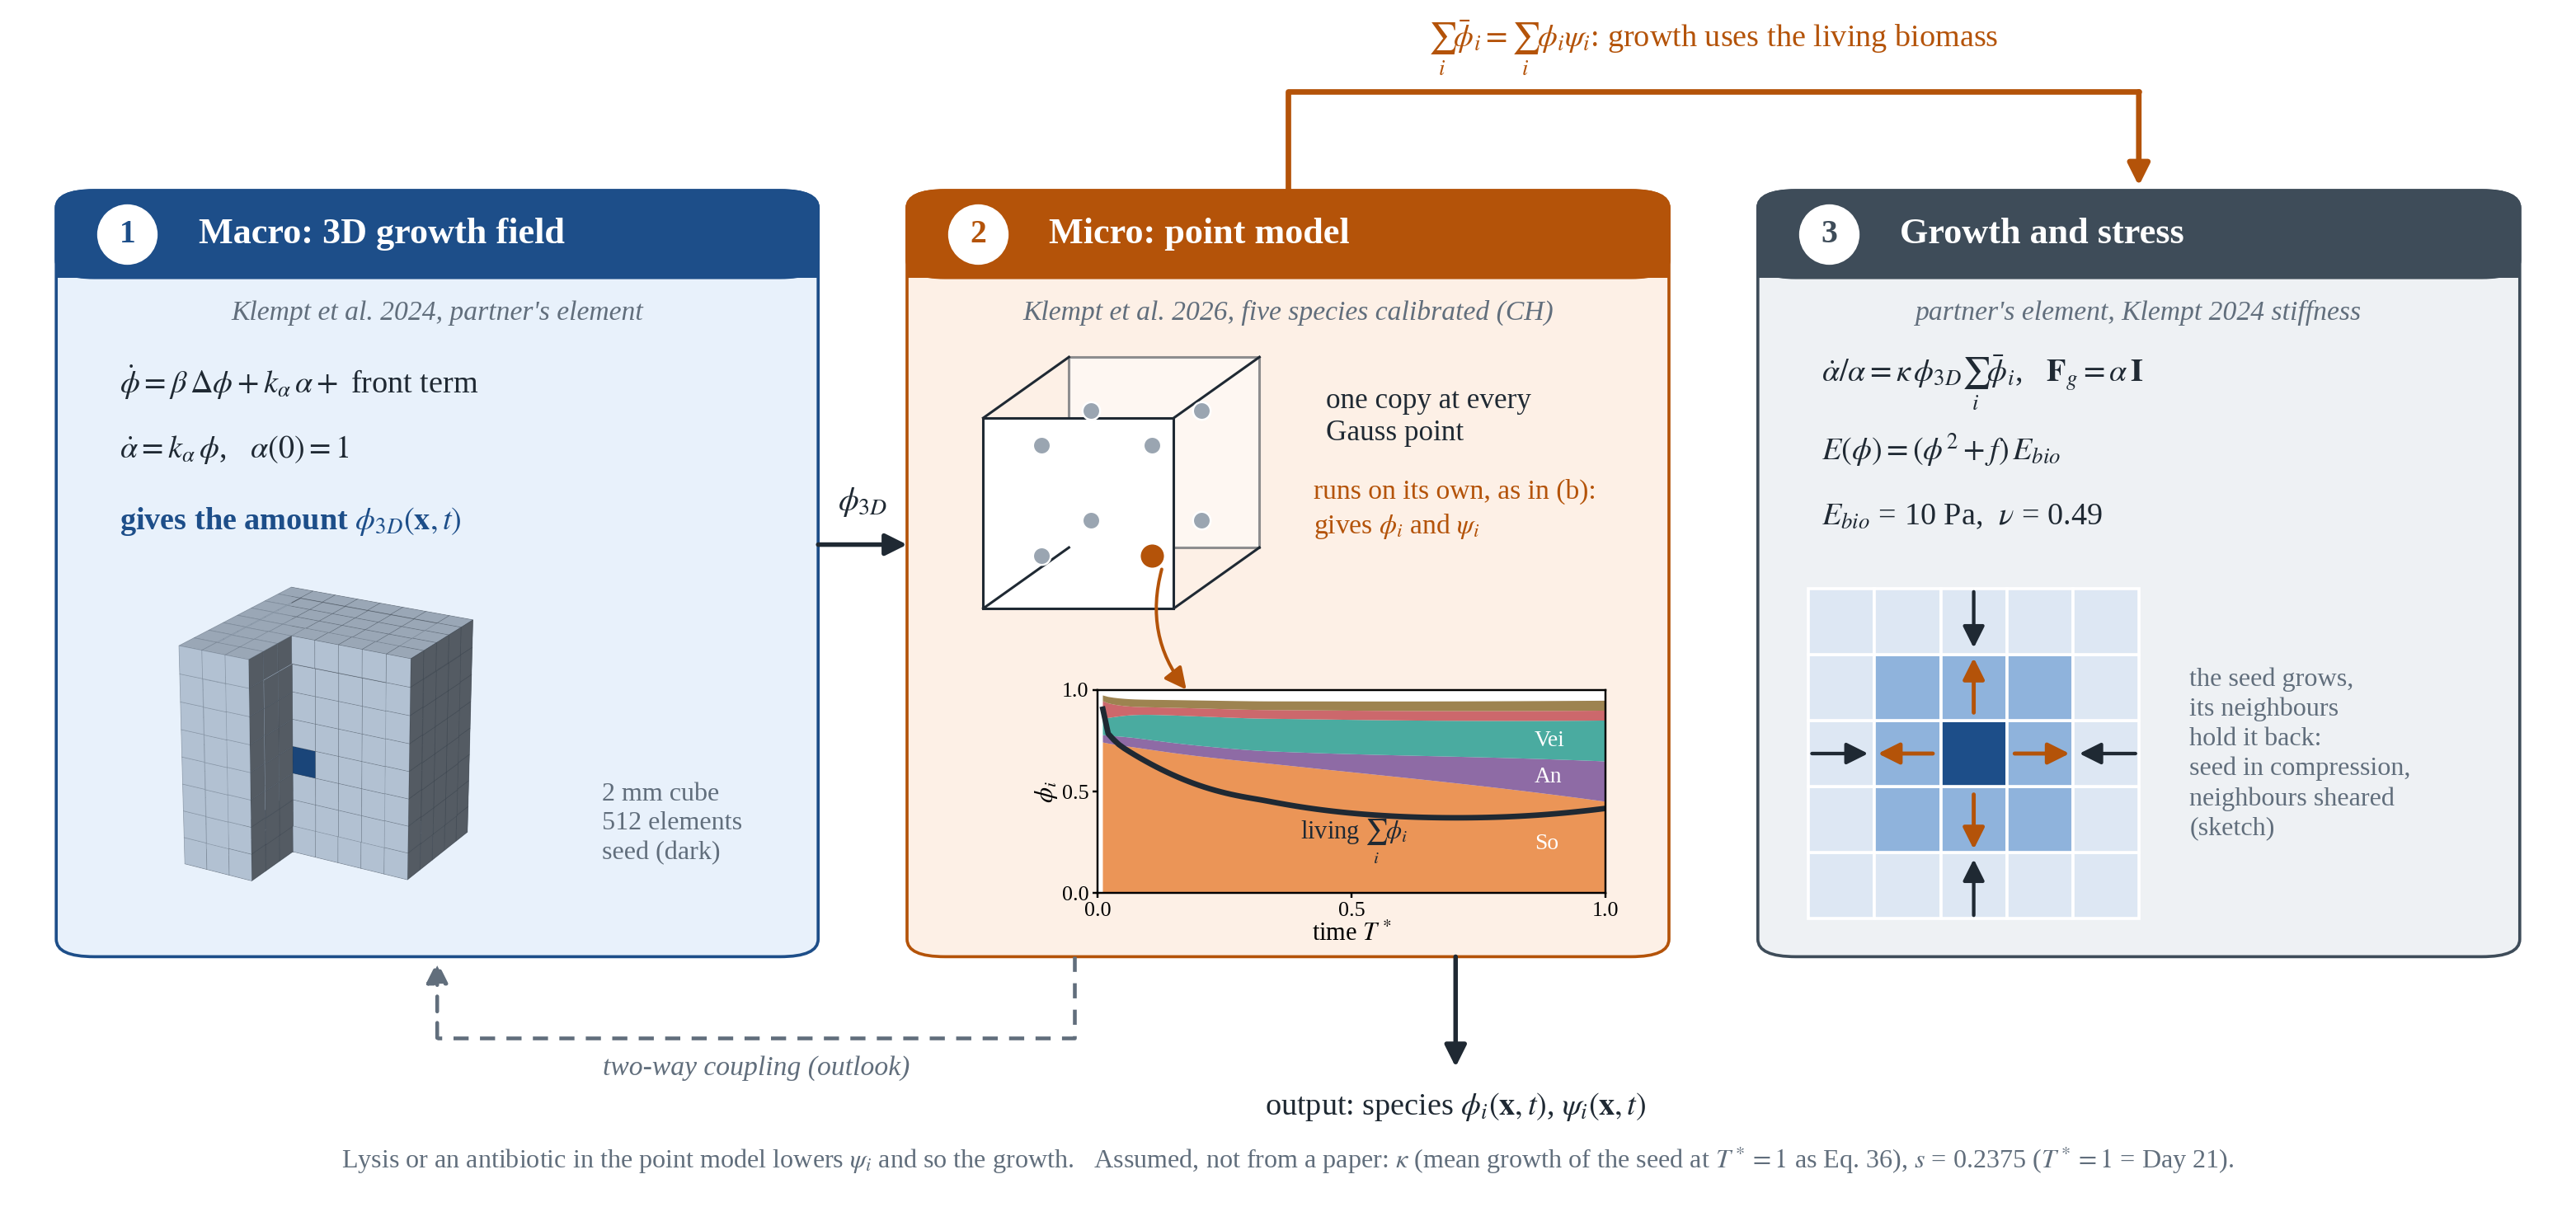
\includegraphics[width=\linewidth]{fig_coupling_schematic_live.png}\\
{\small 方式 (c)：点モデルは生きた割合 $\psi_i$ も決め、成長は生きている量 $\sum_i\bar\phi_i=\sum_i\phi_i\psi_i$ を使う（小さい図：常在・流れの較正済みの計算、シードの Gauss 点）。}

\paragraph{3. 溶菌が成長に効く（方式 (c)）。} 較正した 5 菌種のモデルで、$\alpha$ を $\phi_{3D}$ ではなく
点モデルの生きている量 $\sum_i\bar\phi_i=\sum_i\phi_i\psi_i$ とその場所の量の積で成長させた（$\dot\alpha/\alpha=\kappa\,\phi_{3D}\sum_i\bar\phi_i$）。点モデルは (b) と同じく、縮めずに自分だけで進む。
すると $\psi_i$ が下がる（溶菌、点モデルの中の抗菌薬）と、点モデルの内側から成長が下がる。
$\kappa$ を平均の成長が Eq.~36 と同じになるよう選ぶと、シードの von Mises 応力の平均は $7\,\%$ 低い
（成長の総量は同じで、シードの中の成長の分布が違うため。測定データでの較正で $8^3$ $-7.0\,\%$、16$^3$ $-7.1\,\%$。前の較正では $-7.8\,\%$）。
点モデルに抗菌薬を入れる（全菌種で同じ感受性、$T^*=1$ までに生きた割合が半分になる強さ。どちらも仮定）と、
方式 (c) では成長が $26\,\%$、シードの応力が $32\,\%$ 下がる。方式 (a) では応力は抗菌薬なしと全桁一致し、
組成だけが変わる。成長と応力は $\kappa$ に比例する。$\kappa$ は私が決めた値で、論文の値ではない。

\noindent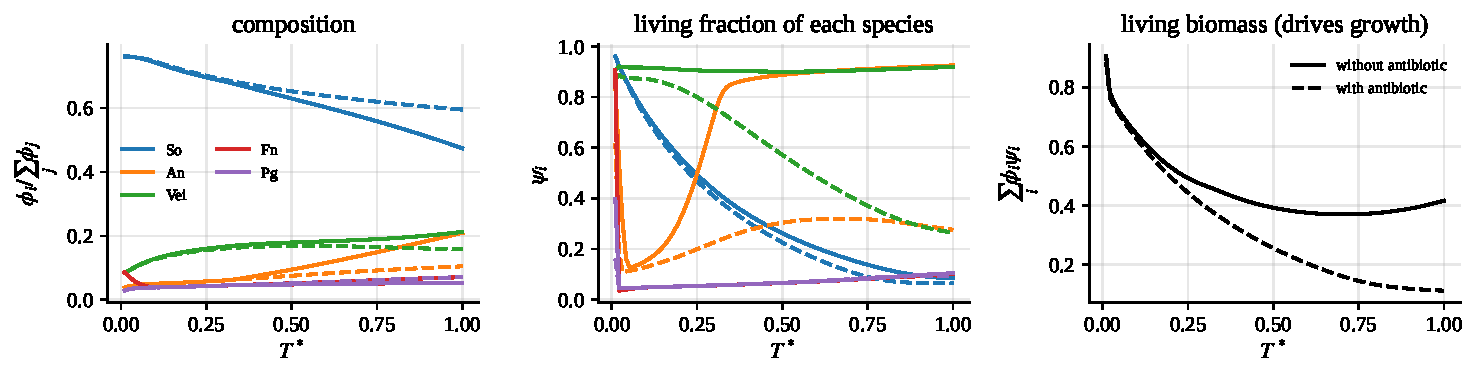
\includegraphics[width=\linewidth]{fig_meeting1019_lysis_trace.pdf}\\
{\small シードの Gauss 点での点モデル、方式 (c)。実線は抗菌薬なし、破線は抗菌薬あり（$T^*=0$ から一定）。
左：組成、中：菌種ごとの生きた割合、右：生きている量（これで成長が決まる）。}

\noindent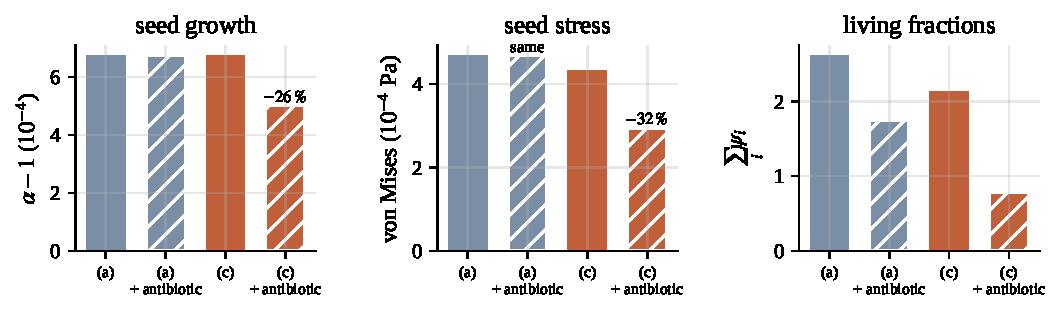
\includegraphics[width=\linewidth]{fig_meeting1019_lysis.pdf}\\
{\small 点モデルの抗菌薬（常在・流れの条件、$8^3$、$T^*=1$、シード要素の平均）。(a) は場の $\phi$ で成長、(c) は生きている量で成長。}

\noindent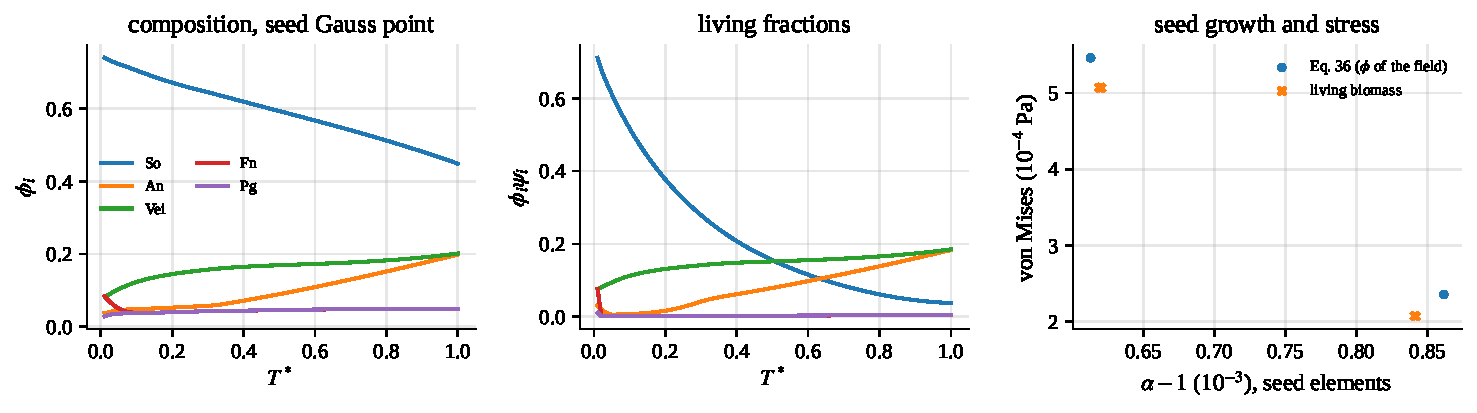
\includegraphics[width=\linewidth]{fig_meeting1019_cal5.pdf}\\
{\small 要素に入れた較正済みの 5 菌種モデル（常在・流れ、$8^3$、$T^*=1$）。シードの Gauss 点の組成と生きた割合、
シード要素の成長と応力（Eq.~36 と、生きている量で成長）。}

\paragraph{抗菌薬を $T^*=0.5$ から入れる。} Fritsch et al.（2025、Fig.~18）の検証のケースと同じく、
抗菌薬を $T^*=0.5$ から入れた。$T^*=0.5$ までは抗菌薬なしと全桁一致し、そのあと成長が遅くなる。
シードの応力は、方式 (a) と比べて：全菌種で同じ感受性なら $16\,\%$ 低い（抗菌薬を強くすると $28\,\%$）。
嫌気性菌（Vei、Fn、Pg）が 10 倍敏感なら $33\,\%$、So だけ敏感なら $19\,\%$ 低い。
方式 (a) は 4 通りとも基準の応力のまま。So は量は多いが、もともと生きた割合が低いので、狙ってもあまり効かない。

\noindent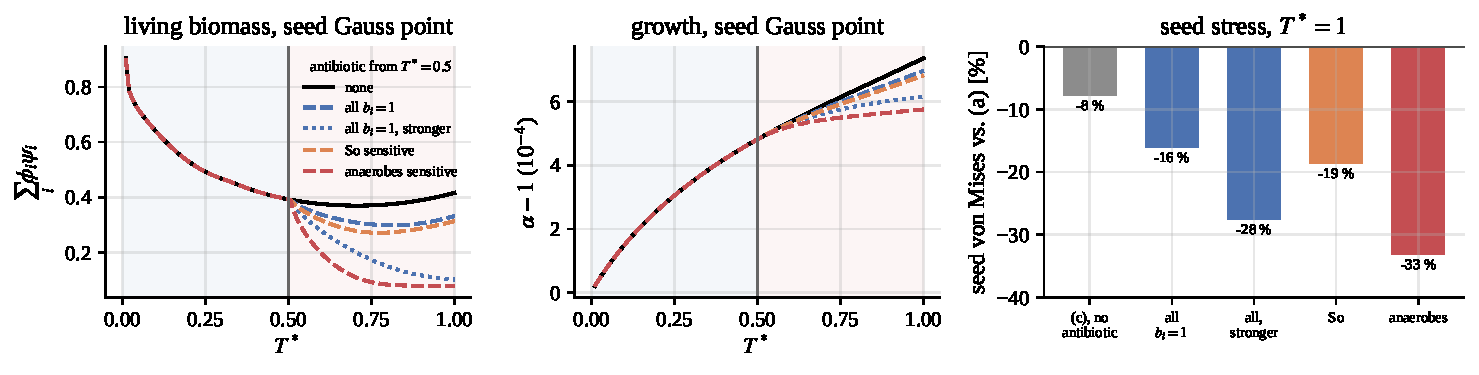
\includegraphics[width=\linewidth]{fig_meeting1019_switch.pdf}\\
{\small $T^*=0.5$ から抗菌薬、方式 (c)、常在・流れ、$8^3$。左と中：シードの第 1 Gauss 点。
右：シード要素の von Mises 応力の平均（方式 (a) との差）。感受性と強さは仮定。}

\par\noindent\begin{minipage}{\linewidth}
\paragraph{比較と提案。}
\begin{center}\small
\begin{tabularx}{\linewidth}{@{}l>{\raggedright\arraybackslash}X>{\raggedright\arraybackslash}X>{\raggedright\arraybackslash}X@{}}
\toprule
& (a) 量で成長 & (b) 独立した点モデル & (c) 生きている量で成長\\
\midrule
何をするか & 量は場、組成は点モデル、$\sum_i\phi_i=\phi_{3D}$ に縮める & 点モデルは自分だけで進み、組成だけ渡す & 点モデルは (b) と同じ。成長は $\dot\alpha/\alpha=\kappa\,\phi_{3D}\sum_i\phi_i\psi_i$\\
$\phi_0$ の意味 & 場の空隙 $1-\phi_{3D}$ & 補助の変数（論文どおり） & (b) と同じ\\
組成を決めるもの & その場所の量 & その場所の年齢 & その場所の年齢\\
溶菌が成長に効くか & 効かない & 効かない & 効く（$\psi_i$ が下がると成長が下がる）\\
確かめたこと & 点モデル単独を $10^{-5}$ で再現 & 点モデルの軌跡が時間でずれるだけ & $8^3$・16$^3$ でシード応力 $-7\,\%$、抗菌薬で $-16$〜$-37\,\%$、(a) は不変\\
修論では & 第 4 章 & 第 4 章、比較として & Outlook に一段落\\
強み & よく確かめてあり、説明しやすい & 論文の $\phi_0$ の読み方に一番近い & 溶菌の問いに答える。生きている量で成長させる例は文献にある\\
弱み & $\phi_0$ に意味を持たせる（仮定として書く） & 場とほとんどつながらない。溶菌を返せない & $\kappa$ は私が決めた値。大きい $\kappa$ では止まる\\
\bottomrule
\end{tabularx}
\end{center}
\noindent\emph{提案：} 修論は (a) を基本、(b) は $\phi_0$ の解釈の比較。(c) は (b) の点モデルのまま生きている量で成長させる形で、溶菌を成長に効かせる発展にする。
\end{minipage}

\paragraph{(a) と (c) のどちらが正しいか。} まだ決まっていない。Klempt et al. 2024 の Eq.~36 は、死んだ菌のない
1 種のモデルの式なので、成長が $\phi$ 全体に従うのか、生きている部分だけに従うのかは決めていない。
生物学としては (c) が自然：体積は生きている菌の分裂と基質（EPS）づくりで増え、古典的なバイオフィルムのモデル
（Wanner と Gujer 1986、Alpkvist と Klapper 2007）も、活性な菌の量だけを成長させる。Heine et al. の体積データでは決められない：
常在・流れの条件では、生きた割合が 0.35〜0.7 まで下がっても体積は増え続け、どちらの方式でも説明できる。
実測の体積の増える部分に、(c) は実測の生きた割合を使い、同じパラメータ数で当てはめると、4 通りすべてで (c) が
少し良いが、差は小さい（$\Delta\chi^2\le0.24$）。Feng et al.（2021）も、各菌種を自分の量に比例して成長させている。
下の実験 1 で決められる：成長の速さを実測の体積（Day~3 から Day~21 で 1.80 倍）に合わせると、途中から嫌気性菌に効く
抗菌薬を入れたとき、(a) は 1.80 のまま、(c) は 1.55 に下がる。

\noindent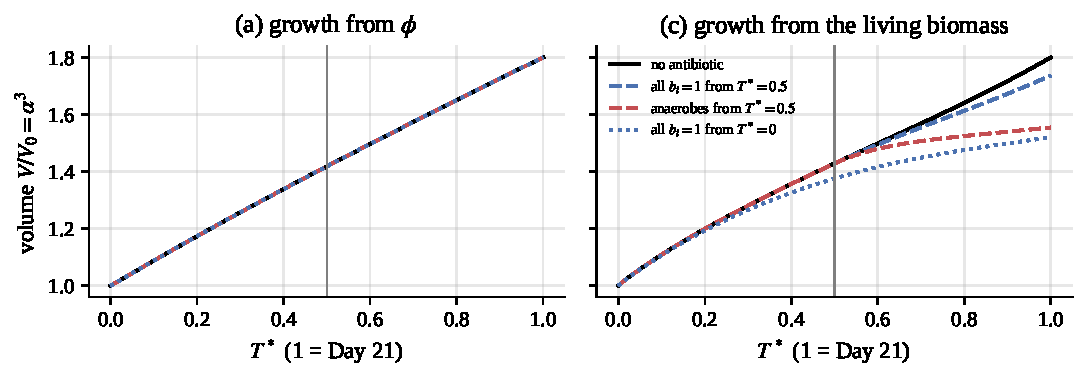
\includegraphics[width=0.8\linewidth]{fig_volume_prediction_antibiotic.pdf}\\
{\small 常在・流れのバイオフィルムの体積の予測（シードの Gauss 点の点モデルから、成長の速さは実測の体積に合わせた。力学は計算していない）。抗菌薬のパラメータは仮定。}

\paragraph{4. 修論に書いた限界。} 力学は一方向の結合（組成は剛性を変えない）。方式 (a) は、点モデルが
意図していない意味を $\phi_0$ に持たせる。こうした選択なしにつなぐには、一つの変分原理から作った、
空間の多菌種モデルが要る。最近の確認：表面の点の $\phi$ は近くの Gauss 点の平均で、一定の場でしか正確でない。
そのため面の近くのラプラシアンには、メッシュを細かくしても減らない誤差がある。私のシードの計算では、
この層が誤差の $0.1$〜$0.2\,\%$ を占める。

\paragraph{モデルを確かめられる実験（アイデアだけ）。}
\begin{enumerate}
\item \emph{成長の途中で 2 種類の抗菌薬。} Heine et al. の 5 菌種のバイオフィルムに、途中から一定の濃度で
  抗菌薬を入れる（Fritsch et al. 2025、Fig.~18 の検証のケースと同じ形）。全体に効く薬（クロルヘキシジン）と、
  嫌気性菌に効く薬（メトロニダゾール：Vei、Fn、Pg に効き、So と An には効きにくい）で 1 回ずつ。
  生きた割合（LIVE/DEAD）と体積（CLSM）を測る。方式 (c) なら、一番多い菌が狙われたときに体積の増え方が落ちる
  ので、薬によって、また常在と dysbiotic で違う。方式 (a) なら、どちらの薬でも体積は変わらない。
  これで二つを決められる。
\item \emph{Fn 抜きの共培養。} dysbiotic の群集を Fn なしで流れの中で育てる。較正したモデルは、後半の Pg の
  増加が消えると予測する。
\item \emph{空間の組成。} FISH と CLSM で、菌種の深さ方向の分布を測る（NIFE に一部ある）。組成を量で決める (a) と
  年齢で決める (b) では分布が違うので、$\phi_0$ の意味の判定になる。
\item \emph{硬さ。} 条件ごと・群集ごとのヤング率を AFM で（Pattem et al. 2018 と同じく）。仮定の $E=10$~Pa を
  置き換える。組成で硬さが変わるなら、両方向の結合の根拠になる。
\item \emph{成長による変形。} 柔らかい基板（ゲルや薄い膜）の上で育て、基板の変形から成長による応力を出す。
  応力を確かめる、今ある中で一番近い方法。
\end{enumerate}
実験をする側へのアイデアとして挙げるだけ。私はコロキウムのあと帰国するので、自分では行わない。1 で (a) と (c) を決められる。

\paragraph{一緒に決めたいこと。}
\begin{enumerate}
\item[] \emph{$\phi_0$ の意味。} 方式 (a) を基本にして、$\phi_0=1-\phi_{3D}$（場の空隙）を仮定として書き、
  (b) を比較にしたい。説明が簡単だから。方式 (c) は点モデルを (b) と同じく動かすので、$\phi_0$ は論文どおり補助の変数のまま。
  つまり今後は論文の読み方を使う。この分け方でよいか、それとも修論でも $\phi_0$ を補助の変数のままにしたいか。
\end{enumerate}

\newpage
\section*{話す順番（20 分、自分用）}
\begin{tabularx}{\linewidth}{@{}l l X X@{}}
\toprule
分 & 内容 & 言うこと（英語） & 意味\\
\midrule
0--2 & 今の状況 & ``The thesis is written; I plan to submit in mid-November. The point model is the Hamilton point model, calibrated by TMCMC, not machine learning.'' & 修論は書き終わった。点モデルは機械学習ではない。\\
2--5 & 1 と 2：二つの空隙 & ``The field and the point model each have their own void. I implemented two ways to match them.'' & 場と点モデルはそれぞれ空隙を持つ。そろえ方を 2 通り作った。\\
5--10 & 3：方式 (c) と抗菌薬 & ``If growth follows the living biomass, an antibiotic lowers the growth and the stress; with my thesis coupling, the stress stays exactly the same.'' & 生きている量で成長させると、抗菌薬で成長と応力が下がる。修論の方式では応力はまったく同じ。\\
10--12 & $T^*=0.5$ から & ``As in Fritsch et al., Fig.~18, the antibiotic is switched on at half time; an antibiotic on the anaerobes lowers the stress most.'' & Fritsch の Fig.~18 と同じく途中から。嫌気性菌に効く薬が一番効く。\\
12--14 & 比較の表と提案 & ``I propose (a) for the thesis, (b) as a comparison, and (c), which keeps the point model of (b), as the extension.'' & 修論は (a)、(b) は比較、(c) は (b) の点モデルを使う発展。\\
14--17 & 決めたいこと & ``Do you agree to state $\phi_0 = 1-\phi_{3D}$ as an assumption in the thesis, while (c) keeps it auxiliary?'' & 修論では $\phi_0$ を場の空隙とする仮定、(c) は補助の変数、でよいか。\\
17--20 & 実験（紹介だけ）と質問 & ``These experiments are only ideas; experiment 1 would decide between (a) and (c).'' & 実験はアイデアだけ。1 で (a) と (c) を決められる。\\
\bottomrule
\end{tabularx}

\vspace{8pt}
\noindent\textbf{最初に聞く 1 問：} 決めたいこと（$\phi_0$ の意味）。修論の第 4 章の書き方に直接かかわるので、
提出（11 月中旬）の前に答えが要る。実験の話は短く、紹介だけでよい。

\vspace{4pt}
\noindent\textbf{聞かれそうなことと答え：}
\begin{itemize}
\item \emph{$\kappa$ はどう決めた？} 平均の成長が Eq.~36 と同じになるように（今の較正で $8.14\times10^{-3}$、前の較正で $8.82\times10^{-3}$）。体積に合わせると約 2.8 だが、
  その値ではシードの外の空の要素がつぶれて $T^*\approx0.35$ で止まる。直す計算を回している。
\item \emph{抗菌薬の値は？} 強さ $\alpha^*$ と感受性 $b_i$ は仮定。較正した $\theta$ の $b$ は全部 0 だった。
\item \emph{なぜ (a) では応力が変わらない？} (a) の成長は場の $\phi$ だけで決まり、$\psi$ を見ないから。
\item \emph{両方向の結合は？} 応力で組成を変える試験は要素で回った。ただし形と値は仮定。文献の「成長を止める圧力」は
  0.1〜1 MPa の桁で、今のモデルの応力（$E=10$~Pa で $10^{-4}$~Pa）より桁で大きい。
\end{itemize}
\end{document}
